\documentclass[UTF8, 11pt, oneside]{ctexart}

\usepackage{float}

\usepackage{geometry}
\geometry{a4paper,left=2cm,right=2cm,top=2cm,bottom=1cm}

\usepackage{graphicx}

\usepackage{hyperref}
\hypersetup{colorlinks=true, linkcolor=red}

\linespread{1.6}


\def\articletitle{金发碧眼和黄毛绿眼之间,差的只是国力}

\usepackage{fancyhdr}
\usepackage{ifthen}
\pagestyle{fancy}
\fancyhf{}
\setlength{\headheight}{14pt}
\fancyhead[R]{\ifthenelse{\value{page}>1}{\thepage}{}}
\fancyhead[C]{\ifthenelse{\value{page}>1}{\articletitle}{}}
\renewcommand\headrulewidth{0pt}

\usepackage{tcolorbox}
\tcbuselibrary{skins}


\newcommand{\zd}[1]{\textbf{\textcolor[RGB]{123,12,0}{#1}}} % 重点

\newcommand{\yh}[1]{% 引用
    \begin{tcolorbox}[enhanced,
        frame hidden, interior hidden,
        before skip = 5mm, left skip=10mm,
        borderline west={5pt}{0pt}{gray!50}]
        #1
    \end{tcolorbox}
}

\newcommand{\biaoti}[1]{% 标题
    \section*{#1}
}

\begin{document}

\begin{center}
    \LARGE{\articletitle\footnotemark}
\end{center}
\footnotetext{
    原文出自公众号“远方青木”的文章 《\href{https://mp.weixin.qq.com/s/giP1VNutGimaZsv_R-eM_w}{\articletitle}》
}

这世界上有一种霸权,叫审美霸权,是文化霸权的一个分支。

审美,是一种意识形态的产物,会根据时代的需要而不断改变。

1840年以前,我们对洋人的外貌描述是“\zd{黄毛绿眼}”,又称罗刹鬼。

这是天朝上国的文化自信,在中国古人的审美体系中西方人就是洋鬼子,外貌如鬼,丑的吓人。

等到了1900年八国联军进北京之后,中国人终于被彻底打服了。

敌视洋人的慈禧,决定量中华之物力,结与国之欢心。

而民间对洋人外貌的描述,也从\zd{黄毛绿眼},改成了\zd{金发碧眼}。

\zd{本来丑如鬼的洋人,突然变得帅气逼人。}

\biaoti{什么是美}

人类对美的定义是在不断变化的。

唐朝以肥为美,汉代以瘦为美,完全相反。

是否存在一个普世的、恒定的、唯一的审美标准呢?

其实也有。

什么叫美?美女和帅哥都有什么特征?

所有人类的潜意识里,都希望能找到最强大最健康的另一半,来传递自己的基因

\zd{而那些能直接判定出一个人是否强大健康的外貌特征,就是美。}

这个原理适用于所有人类种族,甚至适用于自然界中所有物种。

公鸡耗费大量养分发育出了毫无用处的鲜艳鸡冠和羽毛,就是为了以此证明自己是健康而强壮的。

人类世界也是一样。

唐朝物资缺乏,绝大多数人都吃不饱饭,常年处于饥饿状态,肥胖这个外貌特征可以一眼判定你出身富贵人家,同时也代表你是健康的,易生育的。

汉代的强盛时期,已经有很多人能吃饱饭了,尤其是皇宫之内。

这个时候,皇帝就开始追求以瘦为美了,因为青春期的男女都很瘦,年龄大的人基本都会胖。

\zd{瘦这个外貌特征,代表了年轻,所以被追捧。}

而古今中外所有的国家都一致认为,个子高、皮肤细腻有光泽属于美的特征。

这是因为个高的人,大概率会更强壮,更能保护好自己的后代。

而皮肤细腻有光泽,说明你很健康,同时养尊处优,大概率出身富贵人家。

这样的外貌特征,毫无疑问会被认定为美。

而古今中外,\zd{美的定义也一直被皇室和上流社会所把控。}

上流社会认为细腰是美,那细腰就是美。

上流社会认为宽大的帽子和裙子是美,那这就是美。

\begin{figure}[H]
    \centering
    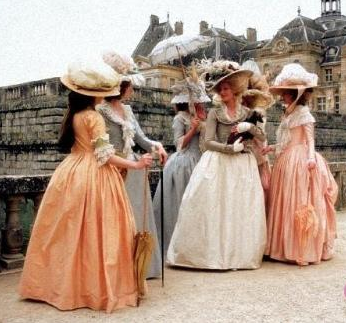
\includegraphics[width=10cm]{2023-09-06-001}
\end{figure}

如果上流社会都拥有这样的外形特征,那社会就会形成一种认知,\zd{拥有这样外形特征的人,大概率就是上流社会。}

而上流社会的人相比普通人而言,更强大,更健康,更有能力抚养好后代。

\zd{所谓美,其实就是性吸引力,强大健康的人更能吸引异性。}

上流社会认可并想拥有的外貌特征,就等于美。

上流社会共有的外形特征,也等于美。

马云穷的时候,丑的像外星人。

当了几年首富后,外貌等级蹭蹭蹭的往上涨,现在看马云就帅多了,潜意识里就认为他不丑,很帅。

甚至那些长的像马云的人,都跟着受益,让人一看就觉得聪明,也挺帅。

\begin{figure}[H]
    \centering
    
\includegraphics[width=10cm]{2023-09-06-002}
\end{figure}

马云的外貌特征,已经成了富裕和强大的代名词。

根据审美观的永恒定律,这种外貌特征自然要被升级为帅的代表。

如果这种外貌特征覆盖的上流社会再多一点,持续时间再久一点。

数百年之后,这就外貌就会替换成为中国文化中的审美观。

\biaoti{本族为美}

我上面说了,美其实就是性吸引力。

\zd{所以任何种族的生物,天生就以本族为美。}

因为本族的异性,才是能让他们基因传递下去的关键。

大猩猩族群里的美人,我相信你不会有任何兴趣。

而大猩猩看人类美女,也不会有什么兴趣。

人类社会的文明中,所有国家和种族都天生拥有强烈的文化自信,\zd{本族最美,异族很丑是一种天生的本能看法。}

科学家的研究发现,不同种族的人对本族人的外貌评价,要明显高于其他种族,我们更倾向于认为那些和我们长的接近的人更好看。

印度人认为本国最牛逼,本族人最好看。

日本人认为本国最牛逼,本族人最好看。

韩国人认为本国最牛逼,本族人最好看。

这是理所当然的事情,\zd{直到他们被打服为止。}

\zd{文化自信崩盘之后,他们就不再认为本族最美了。}

非洲很多部落里,长期将白皮肤和浅色皮肤视为疾病和不健康的象征,是丑陋的表现,黑到发亮的皮肤才是美的代表。

\zd{直到他们被白人统治为止。}

中国古人初见洋人时, 对西方人的外形评价非常的低。

史书是这么记载的:

\yh{赤须碧眼,状如猕猴,形似罗刹。}

用大白话说就是,红毛绿眼,外貌像猴,长得像鬼。

帅?

帅个鬼,丑死人了,和鬼一样。

所以西方人当时还有一个外号,叫洋鬼子。


\biaoti{克拉克玩具娃娃实验}

很多专家在研究人类心理学时,都做过儿童实验。

中国幼儿园的很多小朋友在第一次见到西方人时都非常惊恐,有些甚至会在西方人近距离打招呼时被吓哭,曾有多次实验证实了这一点。

因为小朋友长那么大见到的全是黄皮肤黑眼睛的人,他的世界认知里,拥有这些外貌特征的人,都是安全的,是可以亲热的。

突然见到一个绿眼睛,手臂上有很多毛的人,在小朋友的眼里,这个人形如怪兽,被判定为疑似危险的生物,至少是暂时不能近距离接触的生物。

\zd{这就是幼童最朴素的世界观,是人类的本能。}

但这种本能,是可以被文化改变的。

上世纪40年代,美国心理学家克拉克做了一个实验。

他让一些4~6岁的孩子在一黑一白两个玩具娃娃中选出漂亮的那一个,并询问他们哪个娃娃是好娃娃,哪个娃娃是坏娃娃。

结果不仅白人孩子认为白娃娃好看,是好娃娃,黑娃娃丑陋,是坏娃娃,甚至大部分黑人孩子也这么认为。

在实验录像里,克拉克问一个黑人小女孩:

\yh{“你像哪个娃娃?”}

黑人女孩用手指向黑娃娃,然后犹犹豫豫的说:

\yh{“像那个……坏娃娃。”}

\zd{克拉克玩具娃娃实验说明,在一个白人文化占据绝对主导的社会,即便是刚刚形成自我认知的黑人孩子,都会逆着自己的本能,否定掉自己身边的父母,甚至否定掉自己。}

强势文化会在潜移默化中影响人们的观点和认知,其中当然也包括审美观。

这种现象被称之为文化入侵。

很多人觉得文化入侵是有人编出来吓唬人的,但并不是,\zd{文化入侵是真实存在的。}

白人聪明,黑人蠢。

白人风趣幽默,富有爱心。黑人又脏又乱,喜欢暴力。

哪怕你从未接触过黑人,都会拥有这样的印象。

你见过多少白人,多少黑人?为什么会得出这样的结论?你的这种世界观是自己形成的么?

不,是有人硬生生灌输给你的。

黑人天生就比白人差,哪怕我明面上说和你平等。

凭什么?

就凭白人的种族目前更强大。

\zd{有人可以这么打压黑种人,自然可以这么打压黄种人。 }


\biaoti{丑化中国人}

在国际婚恋市场上,亚裔男的竞争力明显不如亚裔女。

甚至连少量亚裔女,都觉得亚裔男不行。

用的理由并不是没钱,而是没有魅力,她们宁愿找一个穷的白人玩一夜情。

美国主流文化,是相当的看不惯亚裔男人,从各种角度故意丑化和矮化亚裔男性。

大多数美国电影里的中国面孔,\zd{形象都非常不堪,油腻肥胖,邪恶阴险。}

大家可以回忆下看过的美国电影,看看是不是这样,甚至是那些通过审查在中国公映的美国大片,很多时候,也是这样。

亚裔男性扮演的角色,一般就是厨师,书呆子,武打机器,狡猾的中层管理等,通常以反派或丑角据多。

\zd{你见过黄种人面孔的救世主么?}

\zd{你见过善良的黄种人来拯救美国百姓,击败邪恶的白人BOSS的美国大片么?}

你觉得好莱坞会拍这样的电影么?

相当英俊的发哥,参演《加勒比海盗》,给分配的,也是邪恶丑陋的反派角色。

一代男神,被塑造的如此凶狠猥琐。

\begin{figure}[H]
    \centering
    
\includegraphics[width=10cm]{2023-09-06-003.jpg}
\end{figure}

魅力迷人的正面角色,是绝对不可能分配给黄种人扮演的。

而那些毫无性吸引力的反派和丑角,黄种人倒是可以来演一下。

即便是李小龙,成龙这样具有阳刚气息的功夫巨星,也只负责男人之间的肉搏,不会参与到男女之间的感情戏。

一个白人女子被反派掳走,然后被一身正气的迷人黄种人男性李小龙给救出,然后两个人演个半小时的亲亲我我,最终来一个幸福美满的结局。

这样的电影,你听说过吗?

而亚裔女在美国大片里的形象就正面很多,基本都出演美女的角色,虽然大多是花瓶。

\zd{美貌的东方女子,风情万种,迷倒了白人男主,又被坏人掳走,最后白人男主英雄救美。}

这套路,是不是很熟悉?

你以为丑化亚裔很过分?

在中国崛起之前,欧美白人做的更过分,直接把中国男性给邪恶化。

1980年以前,中国人在西方人心目中的形象是被傅满洲系列电影给定型的,这个电影系列频频刷屏,前后拍了14部,每一部都票房爆满,比今天的复仇者联盟热多了。

这个系列的电影,从1921年,一直火到1980年,刷屏半个世纪,可见白人对这个电影的钟爱程度。

\begin{figure}[H]
    \centering
    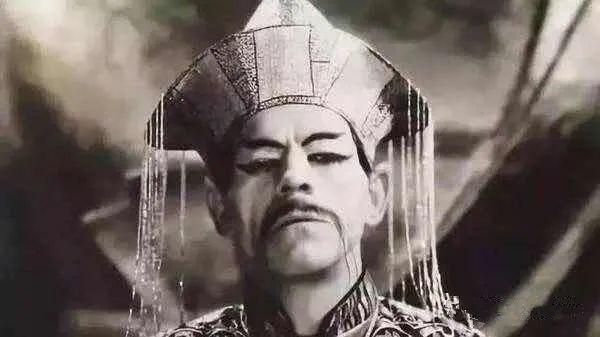
\includegraphics[width=10cm]{2023-09-06-004.jpg}
\end{figure}

中国皇族出身的傅满洲,最喜欢做的事情就是残害白人,虐杀白人女子。

\begin{figure}[H]
    \centering
    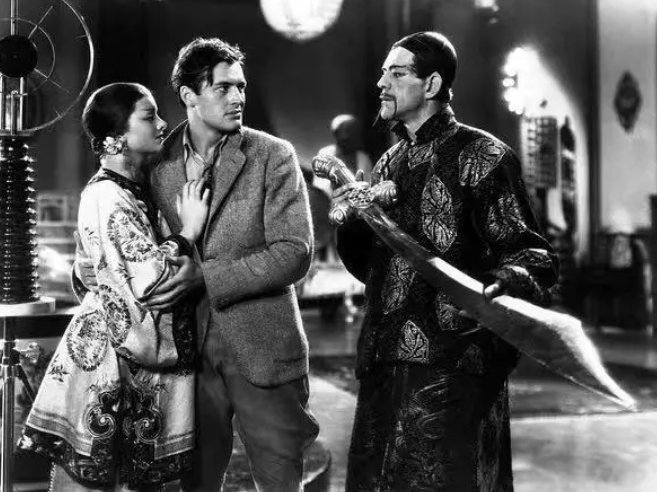
\includegraphics[width=10cm]{2023-09-06-005}
\end{figure}


主演指环王里白巫师的英国国宝级老戏骨克里斯托弗·李,曾在《傅满洲之血》里出演傅满洲。

\begin{figure}[H]
    \centering
    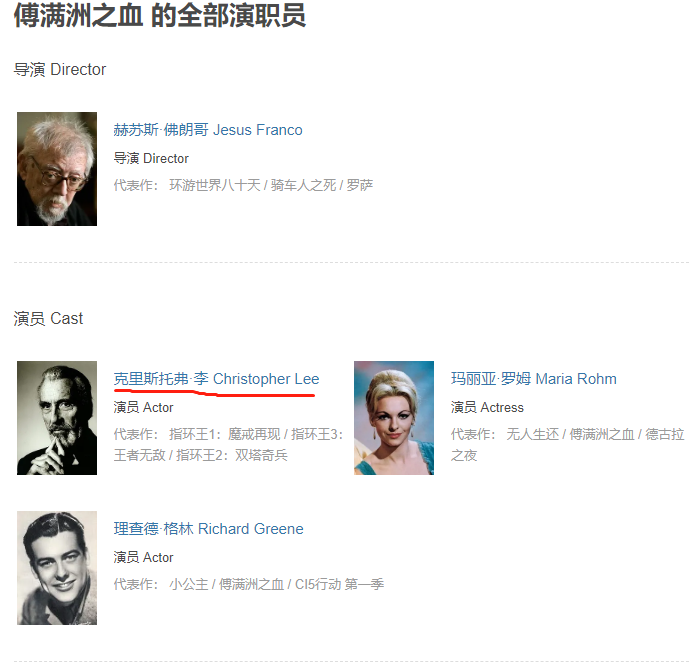
\includegraphics[width=12cm]{2023-09-06-006}
\end{figure}


我们可以从海报图看到,本来长相英俊的克里斯托弗·李,被化妆师故意打扮成了非常丑陋的样子。

\begin{figure}[H]
    \centering
    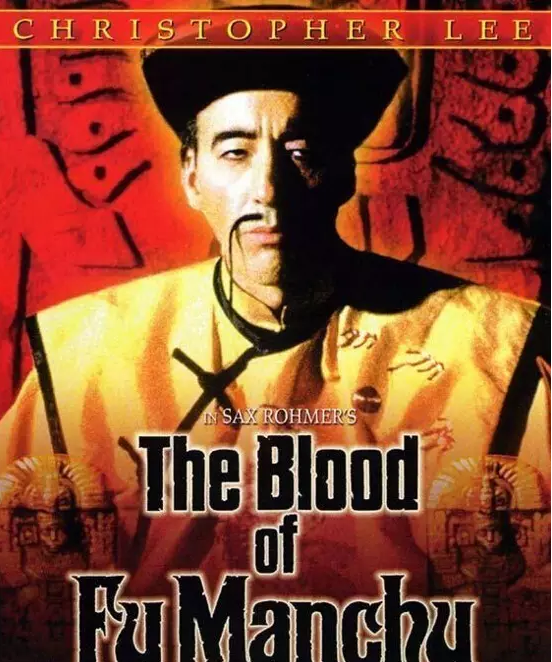
\includegraphics[width=10cm]{2023-09-06-007}
\end{figure}

山羊胡,细长阴冷的眼睛,头戴满清大帽子,留着发辫,聪明狡诈,邪恶狠毒,这就是西方人塑造的中国男人形象。

反正,一看就不是好人那种。

\zd{弘扬中国男性正面形象的美国大片,我没见过,甚至没听说过。}

有研究人员发现,美国荧幕上的亚裔角色,拥有恋爱和家庭关系的概率只有其他族裔的1/4,且绝大多数为亚裔女性和其他族裔男性的组合,整体处于“无性”状态。

这样的美国电影反复轰炸,看电影的人会形成一种什么样的审美观和恋爱观,可想而知。

天下谁不爱慕英雄,\zd{但我见过的英雄,全都长着白人男性的面孔。}

所以在我的眼里,\zd{白人男性的面孔这个外貌特征,就是强大、靠谱、安全感的代名词。}

你觉得,这叫公平吗?

这样的电影看多了,中国人会在潜意识里认为,黄种人或者说中国人就是丑陋的,邪恶的落后人种。而白种人或者说是美国人,就是善良的,英俊的先进人种。

以后美国需要反华的时候,中国人就会一呼百应,放弃抵抗,\zd{默认长着白人面孔的美国“英雄”们,一定会像电影里的那样来拯救我们,赶走坏人。}

这不是文化入侵是什么?


\biaoti{混血优势是谣言}

很多公知和亲西方人士,拼命鼓吹所谓的混血优势。

甚至还有很多媒体,大肆宣传某些漂亮的混血儿,让人们产生混血儿就是聪明漂亮的印象。

\zd{这是自带干粮的美国兵,也是文化入侵潜移默化下的副产品。}

混血优势这个谣言,来源于农作物领域的杂交优势。

袁隆平的杂交水稻,比父本强,比母本也强,拥有极其明显的杂交优势。

但我们要注意了,杂交水稻对父本和母本的选择是极其苛刻的,只有非常特殊的父本和母本杂交,才能获得杂交优势。

\zd{不是随便两款水稻杂交,就会有优势的,那样人人都可以当袁隆平了。}

袁隆平筛选了数万种水稻,才终于找到满意的父本和母本,然后他培育了大量的纯种父本和纯种母本,这样才能批量生产杂交水稻。

大家买宠物狗的时候也应该清楚一个事实,纯种狗的价格,要远远大于血统不纯的杂交狗。

\zd{杂交真的一定有优势,为啥纯血狗卖的那么贵?}

但在公知的洗脑下,很多人真的相信了混血优势这一歪理邪说。

中国美女花大价钱去海外选精,只为了生一个漂亮的“混血宝宝”,这已经不是什么新鲜话题了,很多人这么干。

海外求子甚至在中国已经形成了一个产业链,成为了一个暴利生意。

\zd{崇拜白种人,贬低中国人,无脑向往混血儿的歪风邪气在中华大地上肆虐。}

但实际上,那些被挑出来曝光的混血儿都是千里挑一的特殊品,\zd{大部分混血儿都长残了。}

因为这世界上,根本就不存在混血优势。

真正的混血优势,\zd{应该是混血儿既强于父亲,又强于母亲,}就好像杂交水稻那样。

\zd{如果混血儿只强于母亲的种群,而弱于父亲的种群,那这不叫混血优势,叫母亲的劣质基因污染了父亲的优质基因。}

混血儿弱于父亲的种群,那这个父亲为啥不找一个本族女子,生一个更强的孩子?

\zd{所以拆穿混血优势这个谣言,是非常简单的事情。}

混血优势这个谣言,在全世界都很普及。

\zd{但只有种族自卑的人,才会大力鼓吹混血优势论,}认为混血可以改善本民族的劣质基因。

\zd{而种族自信的人,会非常排斥混血论,}认为混血儿都是低等的,是又笨又丑的,以防止劣等基因混入自己民族的血脉。

希特勒绝对不会认为日耳曼人和犹太人混血会产生更强的后代,他对这种混血儿的态度可以总结为:\zd{劣等,恶心,杂种,污染源。}

处理态度就一个字,杀。

如果白种人和黄种人的后代,真的具有混血优势,真的比父亲和母亲都要强。

那来中国求婚的白种男人和想嫁到中国的白种女人,应该排几万米的长队,毕竟拥有更强的后代是人类的天性。

但实际上我们可以看到,白种人优先选择的结婚对象是本族白人,对和黄种人结婚是非常排斥的事情。

混血优势论在白人那里毫无市场,\zd{他们信奉的是纯种优势论,混血劣势论。}

如果白人认为混血会破坏自己的基因,生下的是混血杂种,而中国人认为混血会增强自己的基因,生下的是混血天使。

那请问,混血真的一定有优势吗,为何白人不想要这种优势宝宝?

那些鼓吹混血优势的公知们,鼓吹的其实是白人基因优势论,而不是什么混血优势,默认中国人基因劣等,内心极度自卑。

否则的话他们为什么不找一个和黑人混血的宝宝照片,然后大夸特夸,哇真漂亮,长大了一定很聪明,混血儿都是聪明又漂亮的。

他们没有这么做,他们只认为和白人混血,才能生出漂亮的优势宝宝。

\zd{可惜,白人不这么认为。}

古人都知道送女子和亲是可耻的行为,但现在有些人干的龌龊事,连古代的卖国贼都不如。

不得不感慨,文化洗脑真的太可怕了,\zd{能让你主动送上门献身的文化入侵,真的比刀枪还厉害。}


\biaoti{种族自信需要国力支撑}

既然文化入侵这么可怕,那我们怎么来抵御文化入侵,甚至反守为攻?

是不是大力培养文艺天才就可以了?

你错了,\zd{文艺天才有用,但没有大用。}

梅兰芳这样的文艺大师,哪怕出100个也只能缓解文化入侵,断然不可能反守为攻。

\zd{种族自信,需要国力的支撑。}

1840年之前,中国人是相当的自信,西方人没有一丝可能发动文化入侵。

浑身体毛,大鼻子,蓝眼睛,一身黄毛的西方人,那就是罗刹鬼啊,咋文化入侵?

但是100年之后,西方人已经成为了强大的代名词,因为中国战败了。

\zd{而强大的种族,其外貌特征一定会成为美的代名词,这是由人类审美观的本质决定的。}

洋人就是英俊潇洒,在这100年里形成整个中国默认的事实。

甚至连建国后官媒拍摄的电影,里面出现的外国人形象,都要采用高大英俊的西方男人来出演,因为这样拍出来才感觉“符合历史”。

虽然有意识的把义律拍的邪气了一点,但依然很英俊。

\begin{figure}[H]
    \centering
    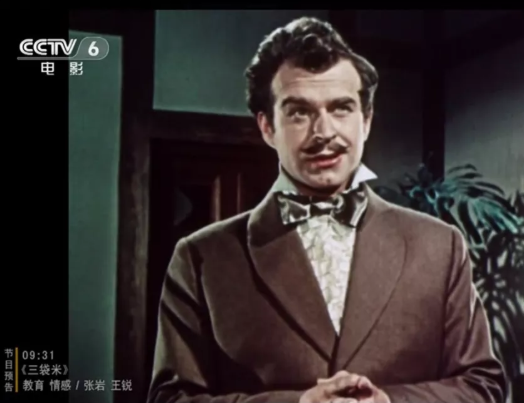
\includegraphics[width=10cm]{2023-09-06-008}
\end{figure}

但下面这个也是白人男性,我们为什么就不能找一个这样的人来演义律,和林则徐搭对台戏呢?

\begin{figure}[H]
    \centering
    
\includegraphics[width=10cm]{2023-09-06-009.jpg}
\end{figure}

美国电影里的华裔男子,十之八九都是由中年肥胖的黄种男人出演,奸诈狡猾,小算盘打的噼啪响。

这种手法,为什么我们不参考?

\zd{因为国力不足,种族自卑,所以文化必然自卑,没办法参考。}

在中国5000多年的历史中,外国人的长相有4900年是和鬼一样的。

除了被坚船利炮给打服的那100年。

罗马横扫欧洲的时候,整个欧洲的人都在学习罗马的一切,罗马贵族的装扮和用品受到欧洲人热烈的追捧。

而中国成为亚洲霸主的时候,日本人和韩国人,连中国的筷子都学。

你们的餐具都是野蛮落后的,中国人的筷子才是先进文明的。

为啥中国的筷子就一定代表先进文明?

这不废话么,中国那么强,当然一切都是文明和先进的,还需要理由?

\zd{你强,你啥都好,别人看你啥都是完美的。}

\zd{你不强,连自己的国人都开始拿起刀叉故弄风雅。}

一般来说,霸权欺凌都有一个实施主体。

但文化霸权和审美霸权并没有,他没有主体,不是个人发动,也不是国家发动,而是一种无意识的存在,\zd{是阶层对阶层的霸权,或者种族对种族的霸权。}

文化的基础是经济地位和社会地位,\zd{富裕的国家可以轻而易举的输出自己的观念和审美标准,以此影响其他种族。}

所以我们要抵御文化入侵,甚至反守为攻,最需要提升的,是国力。

\zd{国力强盛了,种族天然就自信了。}

\zd{金发碧眼和黄毛绿眼之间,差的只是国力。}

但是在国力强盛之前,\zd{我们普通人还可以做一些其他的事情,比如说科普,比如说辟谣,}尽最大努力拖延他国文化入侵的脚步。

比如说那种海外求精生漂亮混血宝宝的害人谣言,就必须予以清除,以正视听。

一个自认基因劣等的民族,白人是不屑于和你通婚的,因为别人不想被你的基因给污染,最后你也只能掏钱买精。

只要我们拖延了文化入侵和洗脑的攻势,那我们的国力就会逐步提升,最终反超。

等国力反超之后,我们就可以在文化领域,反守为攻。

\zd{曾经的黄毛绿眼,因为坚船利炮变成了金发碧眼。}

\zd{但我相信,金发碧眼会在未来的某一天,再度变成黄毛绿眼。}

\end{document}

